%@descr: wzór sprawozdania, raportu lub pracy - nadaje się do przeróbek
%@author: Maciej Komosiński

\documentclass{article} 
\usepackage{polski} 
\usepackage[utf8]{inputenc} 
\usepackage[OT4]{fontenc} 
\usepackage{graphicx,color} %include pdf's (and png's for raster graphics... avoid raster graphics!) 
\usepackage{url} 
\usepackage[pdftex,hyperfootnotes=false,pdfborder={0 0 0}]{hyperref} %za wszystkimi pakietami; pdfborder nie wszedzie tak samo zaimplementowane bo specyfikacja nieprecyzyjna; pod miktex'em po prostu nie widac wtedy ramek


% Zmiana rozmiarów strony tekstu
\addtolength{\voffset}{-1cm}
\addtolength{\hoffset}{-1cm}
\addtolength{\textwidth}{2cm}
\addtolength{\textheight}{2cm}

%bardziej zyciowe parametry sterujace rozmieszczeniem rysunkow
\renewcommand{\topfraction}{.85}
\renewcommand{\bottomfraction}{.7}
\renewcommand{\textfraction}{.15}
\renewcommand{\floatpagefraction}{.66}
\renewcommand{\dbltopfraction}{.66}
\renewcommand{\dblfloatpagefraction}{.66}
\setcounter{topnumber}{9}
\setcounter{bottomnumber}{9}
\setcounter{totalnumber}{20}
\setcounter{dbltopnumber}{9}

% własny bullet list z malymi odstepami
\newenvironment{tightlist}{
\begin{itemize}
  \setlength{\itemsep}{1pt}
  \setlength{\parskip}{0pt}
  \setlength{\parsep}{0pt}}
{\end{itemize}}

%obrazkow szukamy w nastepujacym katalogu:
\graphicspath{{pics/}}



%\title{Sprawozdanie z laboratorium:\\Metaheurystyki i Obliczenia Inspirowane Biologicznie}
%\author{}
%\date{}


\begin{document}

\thispagestyle{empty} %bez numeru strony

\begin{center}
{\large{Sprawozdanie z laboratorium:\\
Metaheurystyki i obliczenia inspirowane biologicznie}}

\vspace{3ex}

Część I: Algorytmy optymalizacji lokalnej, problem ATSP
%Część II: Algorytmy optymalizacji lokalnej i globalnej, problem QAP
%Część III: Eksperyment: ... (prezentację można zrobić w LaTeX - służy do tego klasa "beamer")

\vspace{3ex}
{\footnotesize\today}

\end{center}


\vspace{10ex}

Prowadzący: dr hab.~inż. Maciej Komosiński

\vspace{5ex}

Autorzy:
\begin{tabular}{lllr}
    \textbf{Marcin Mrugas} & inf122580 & marcin.mrugas@student.put.poznan.pl \\
    \textbf{Piotr Kicki} & inf122401 & piotr.kicki@student.put.poznan.pl \\
\end{tabular}

\vspace{5ex}

Zajęcia środowe, 16:50.

\vspace{35ex}

\noindent Oświadczam/y, że niniejsze sprawozdanie zostało przygotowane wyłącznie przez powyższych autora/ów,
a wszystkie elementy pochodzące z innych źródeł zostały odpowiednio zaznaczone i~są cytowane w bibliografii.  

\newpage


\section*{Udział autorów}
\begin{tightlist}
\item MM zaimplementował szkielet aplikacji, oraz przeszukiwanie losowe, przeprowadził eksperyment..., opisał..., przygotował...
\item PK zaimplementował przeszukiwanie zachłanne..., przeprowadziła eksperyment..., opisała..., przygotowała...
\end{tightlist}






\section{Wstęp}

Naszym zadaniem było zaimplementowanie i przestudiowanie asymetrycznego problemu komiwojażera. Problem ten polega na znalezieniu najkrótszego cyklu Hamiltona w grafie asymetrycznym. Można go interpretować jako logistyczny problem dotyczący znalezienia takiej trasy dla dostawcy, aby ten odwiedził wszystkich odbiorców w jak najkrótszym czasie. Problem należy do klasy problemów NP-zupełnych. Złożoność tego problemu, w najgorszym przypadku, sprowadza się do przeglądnięcia wszystkich cyklów Hamiltona których dla grafu o zupełnego o $n$ wierzchołkach jest $n!$. Dlatego problem ten optymalizuje się algorytmami które w przestrzeni rozwiązań starają się rozważać mniejszą część rozwiązań i uzyskują rozwiązania często gorsze od optymalnego ale osiągają ten wynik w znacznie krótszym czasie.

\begin{figure} 
\begin{center}
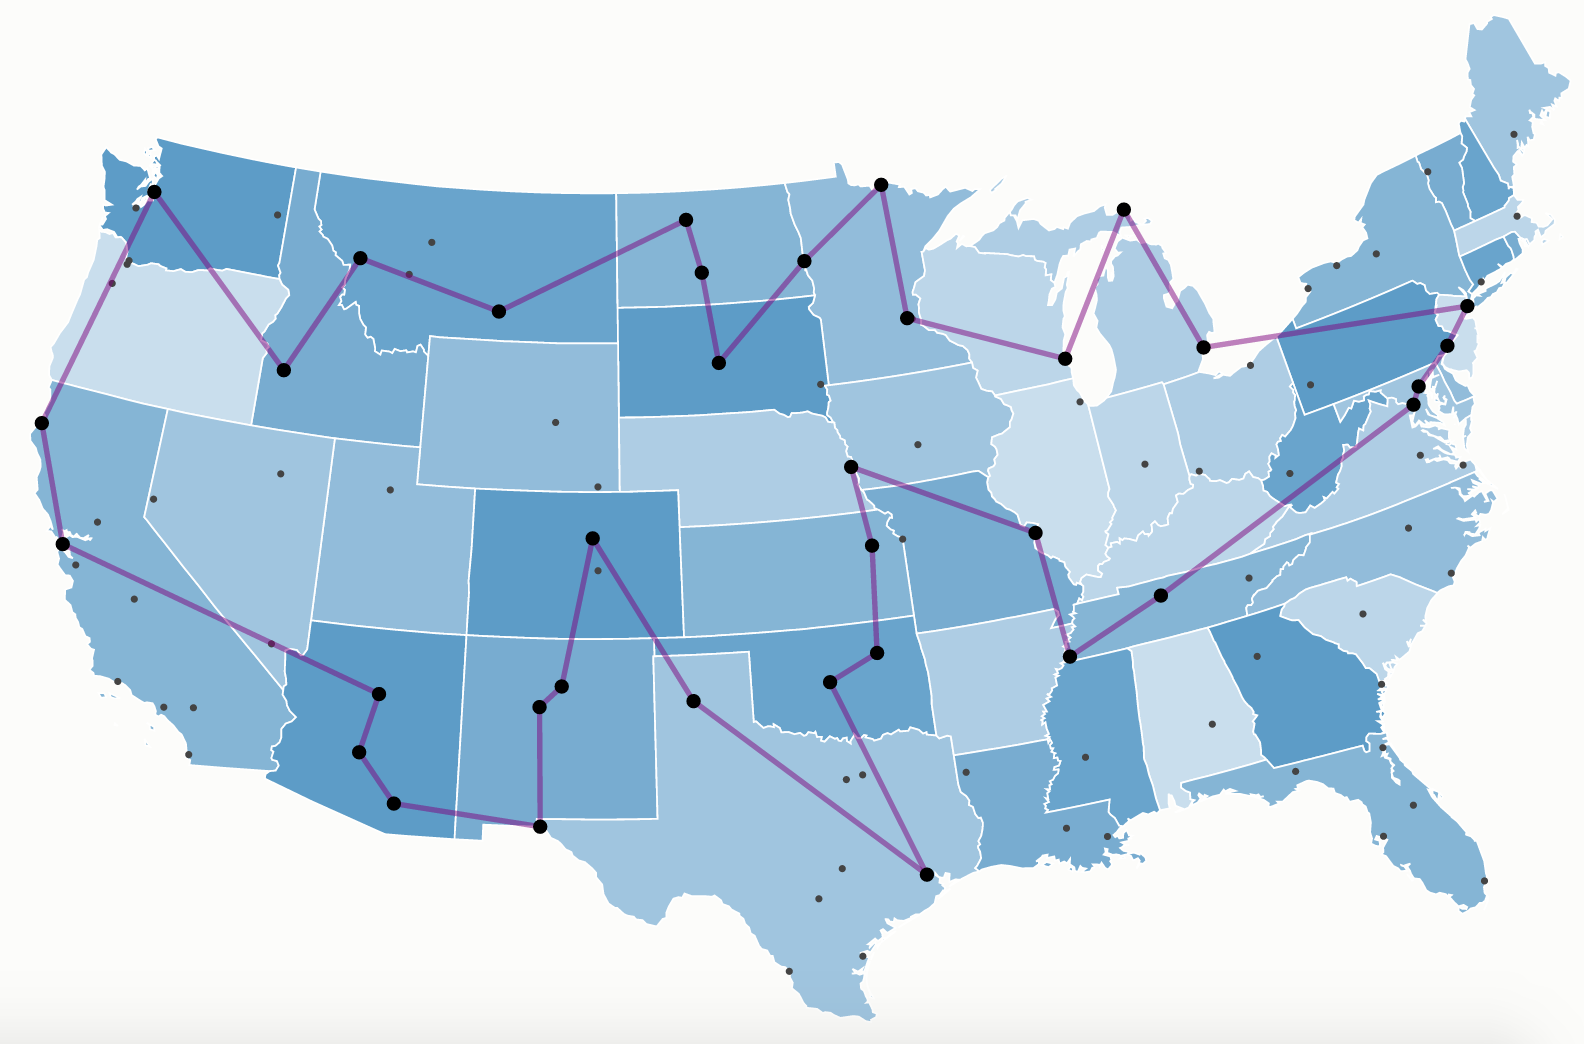
\includegraphics[width=0.7\textwidth]{TSP_USA.png}
\end{center}
\caption{Przykładowe rozwiązanie problemu komiwojażera polegającego na znalezieniu trasy pomiędzy stolicami stanów Stanów Zjednoczonych.}
\label{fig:schemat}
\end{figure}


\section{Opis sąsiedztwa}

Operatorem sąsiedztwa w naszej implementacji jest 2-OPT. Nowy sąsiad jest tworzony poprzez zamianę miejscami dwóch wierzchołków rozwiązania. 

\begin{figure} 
\begin{center}
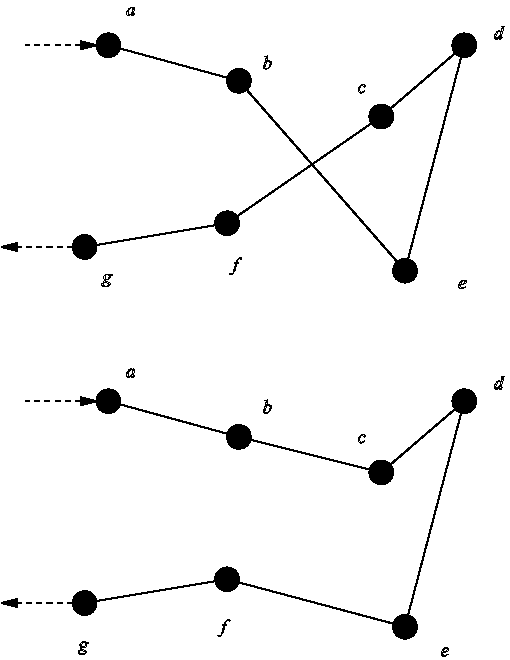
\includegraphics[width=0.4\textwidth]{twooptwiki.pdf}
\end{center}
\caption{Przykład sąsiedztwa.}
\label{fig:schemat}
\end{figure}


\section{Porównanie działania algorytmów}


\subsection{Jakość}
Za miarę jakości obraliśmy wartość równania:
$$ \frac{\eta}{\eta_{min}}-1 $$
gdzie:\\
$\eta_{min}$ -- długość optimum globalnego \\
$\eta$ -- długość rozważanego rozwiązania

Co można interpretować jako wartość o ile długość rozwiązania $\eta$ jest procentowo dłuższa od rozwiązania optymalnego $\eta_{min}$

\begin{figure}[h!]
\begin{center}
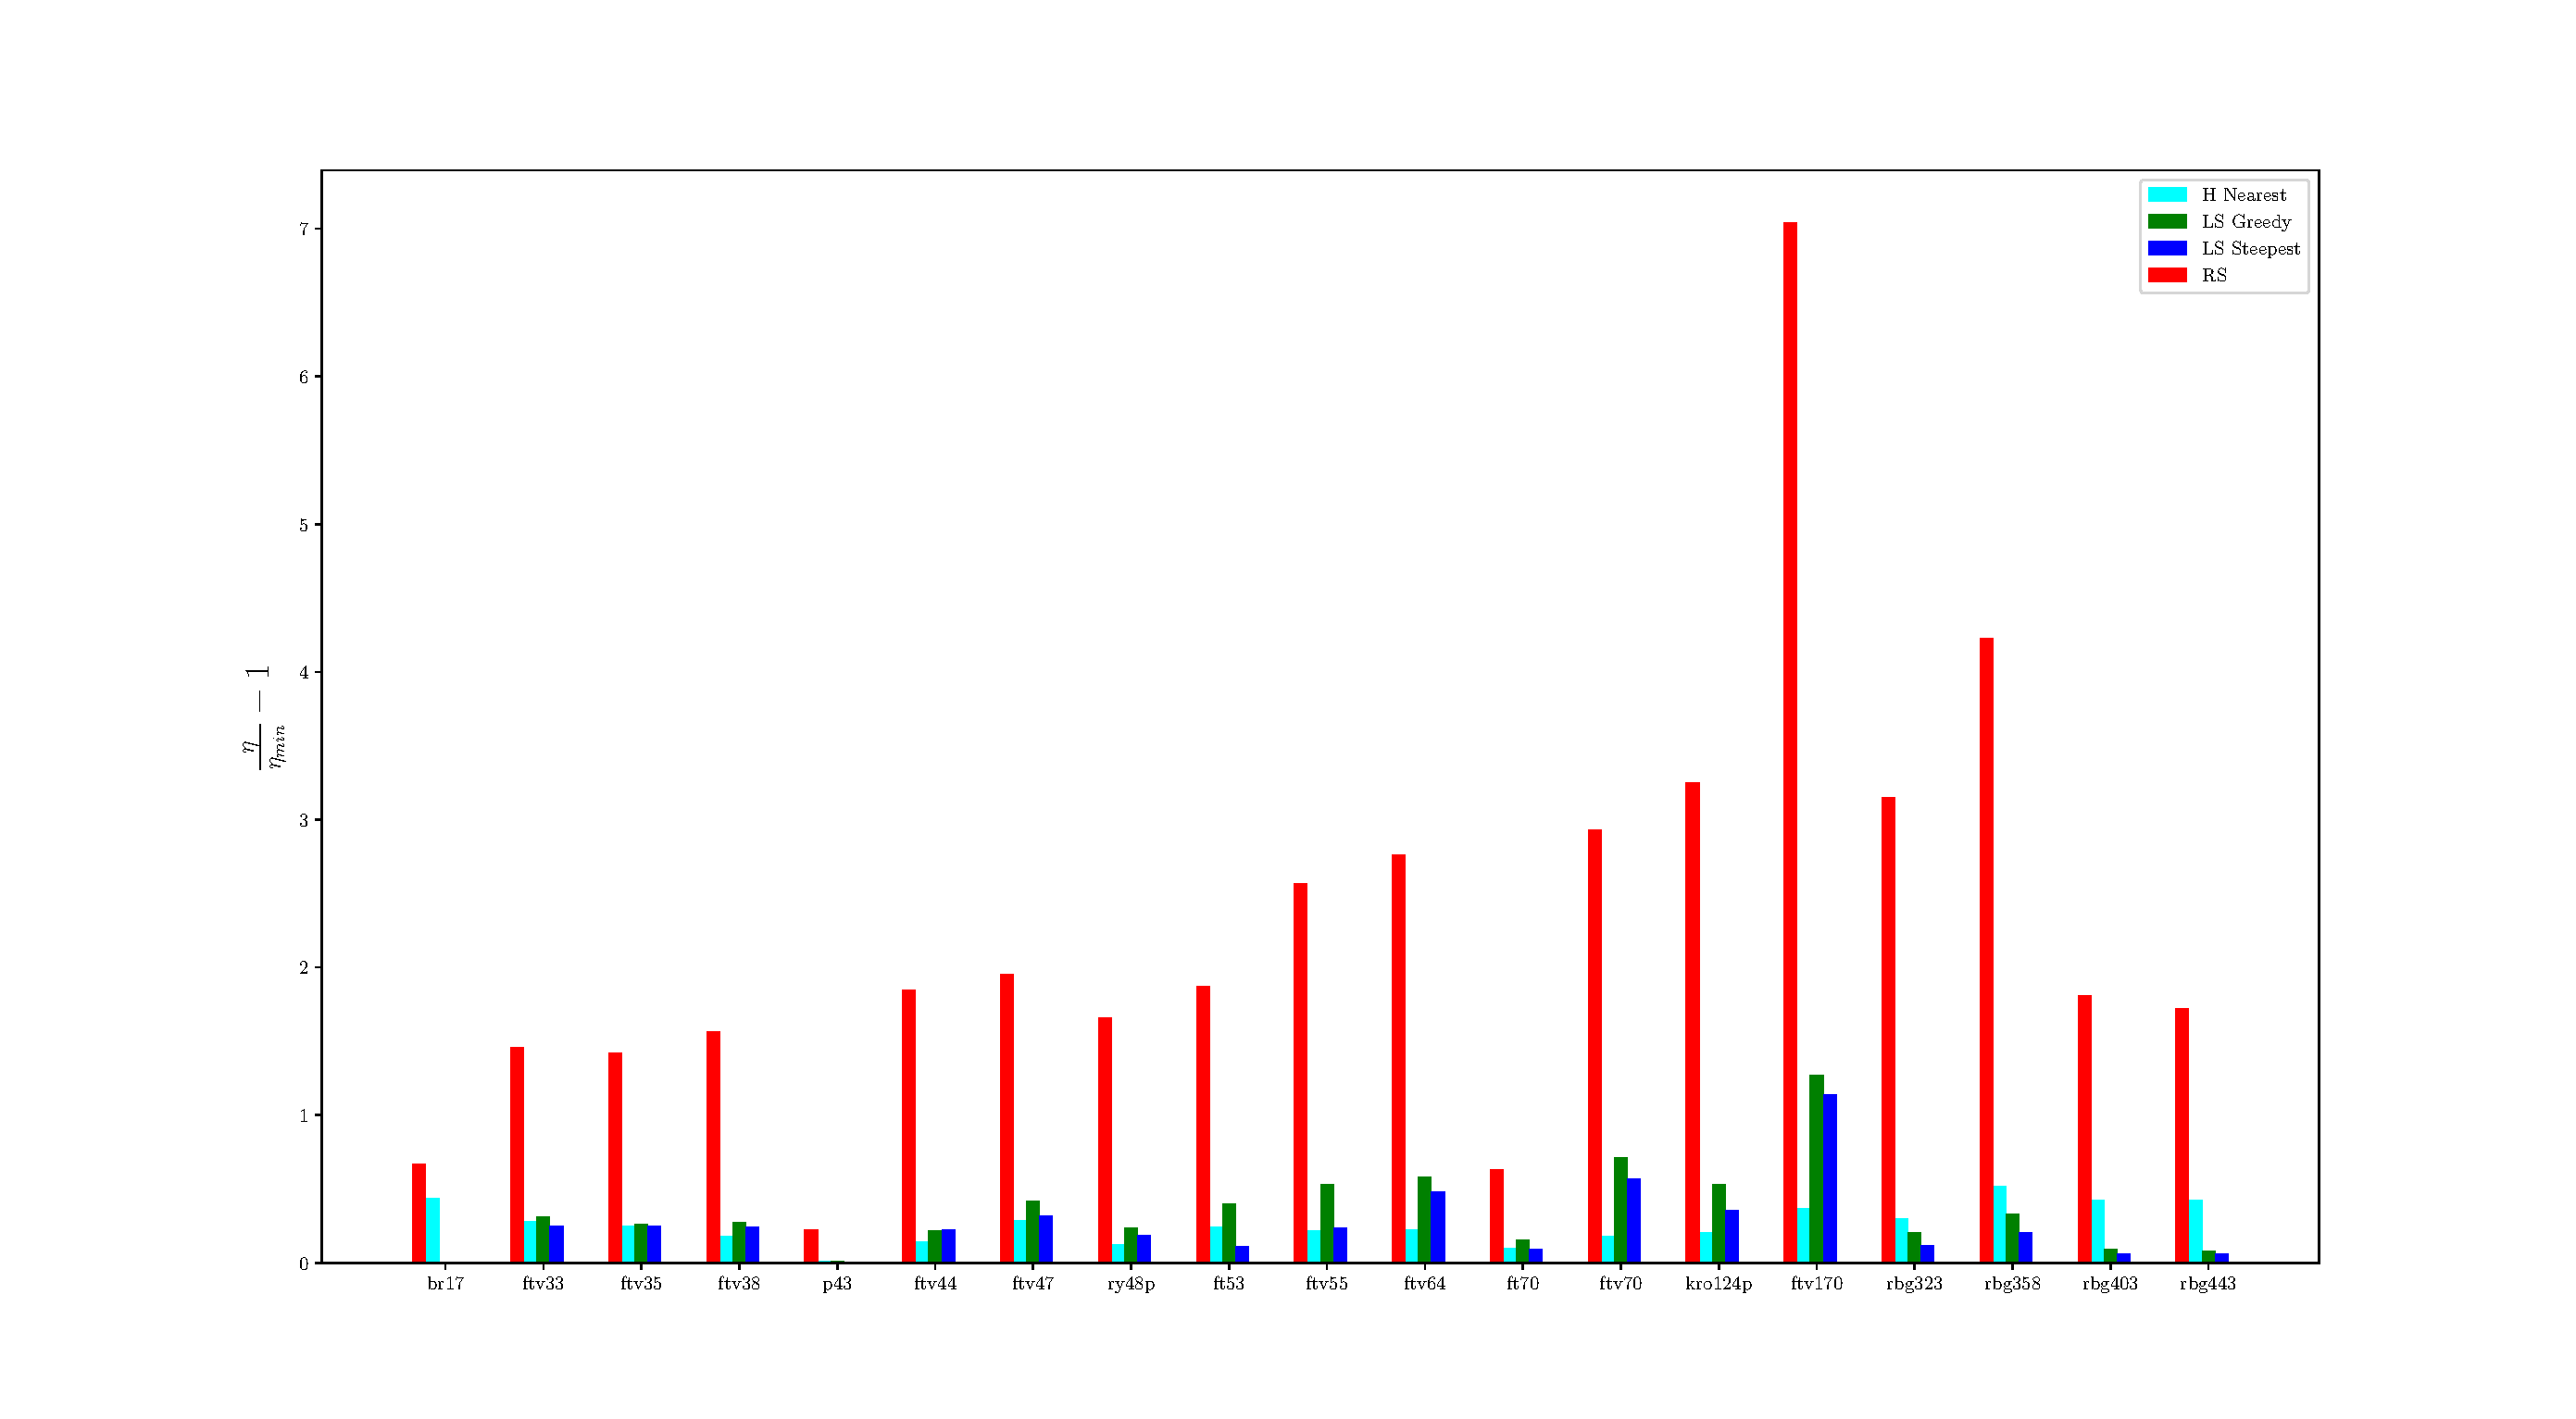
\includegraphics[width=1\textwidth]{min_s.pdf}
\end{center}
\caption{Najlepsze uzyskane wyniki.}
\label{fig:plot_min}
\end{figure}

Na rys. \ref{fig:plot_min} przedstawiono wykres zawierający najlepsze wyniki z 10 uruchomień algorytmów. Na wykresie można zauważyć że najgorsze wyniki daje algorytm Random Search, który uzyskuje średnio jakość 1 - 2 czyli dwukrotnie gorsze rozwiązanie od optymalnego oraz 8 razy gorsze w najgorszym przypadku. Pozostałe algorytmy dawały bardzo podobne do siebie rezultaty czyli o 30\% gorsze od rozwiązania optymalnego.


Na rys. \ref{fig:plot_svg} zostały przedstawione średnie wyniki algorytmów.

\begin{figure} 
\begin{center}
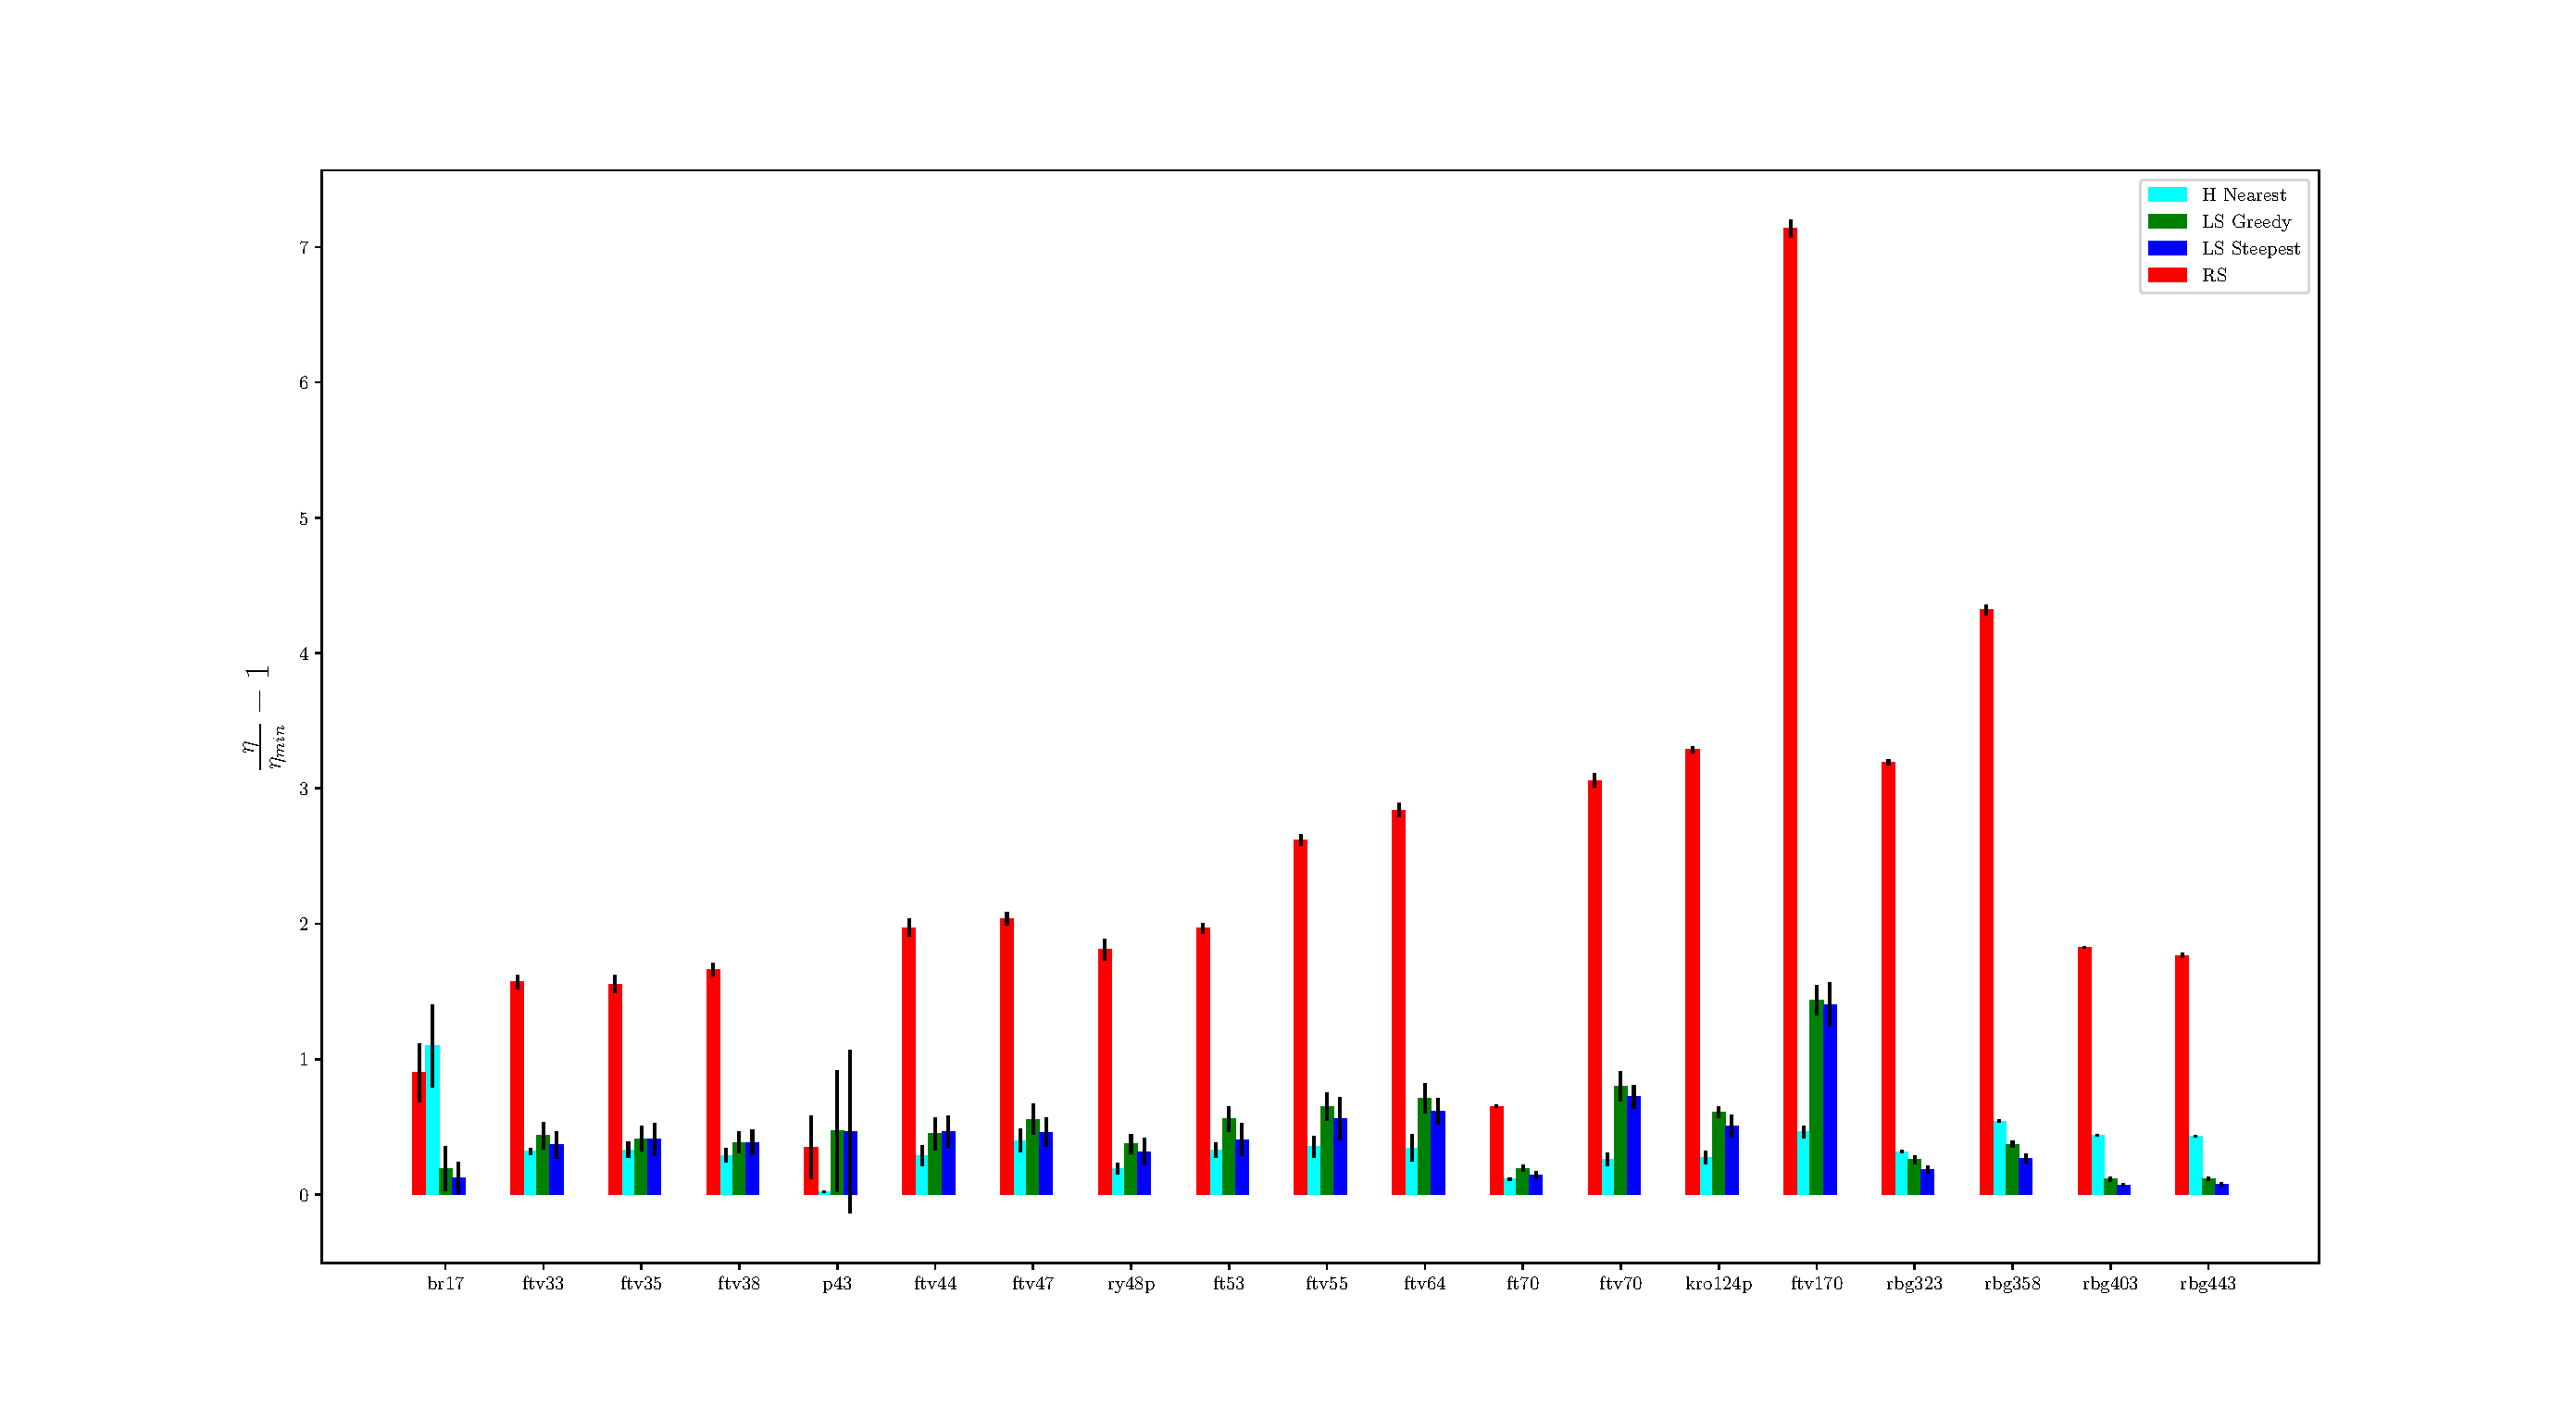
\includegraphics[width=1\textwidth]{avg_s.pdf}
\end{center}
\caption{Średnie wyniki algorytmów}
\label{fig:plot_avg}
\end{figure}

\subsection{Czas działania}

Rys. \ref{fig:plot_time} Przedstawia czas działania algorytmów. Naszybciej działał algorytm heurystyczny, następnie Greedy i na końcu Steepest. Czas działania algorytmu losowego był dobrany tak aby działał porównywalnie długo jak algorytm lokalny.

\begin{figure} 
\begin{center}
    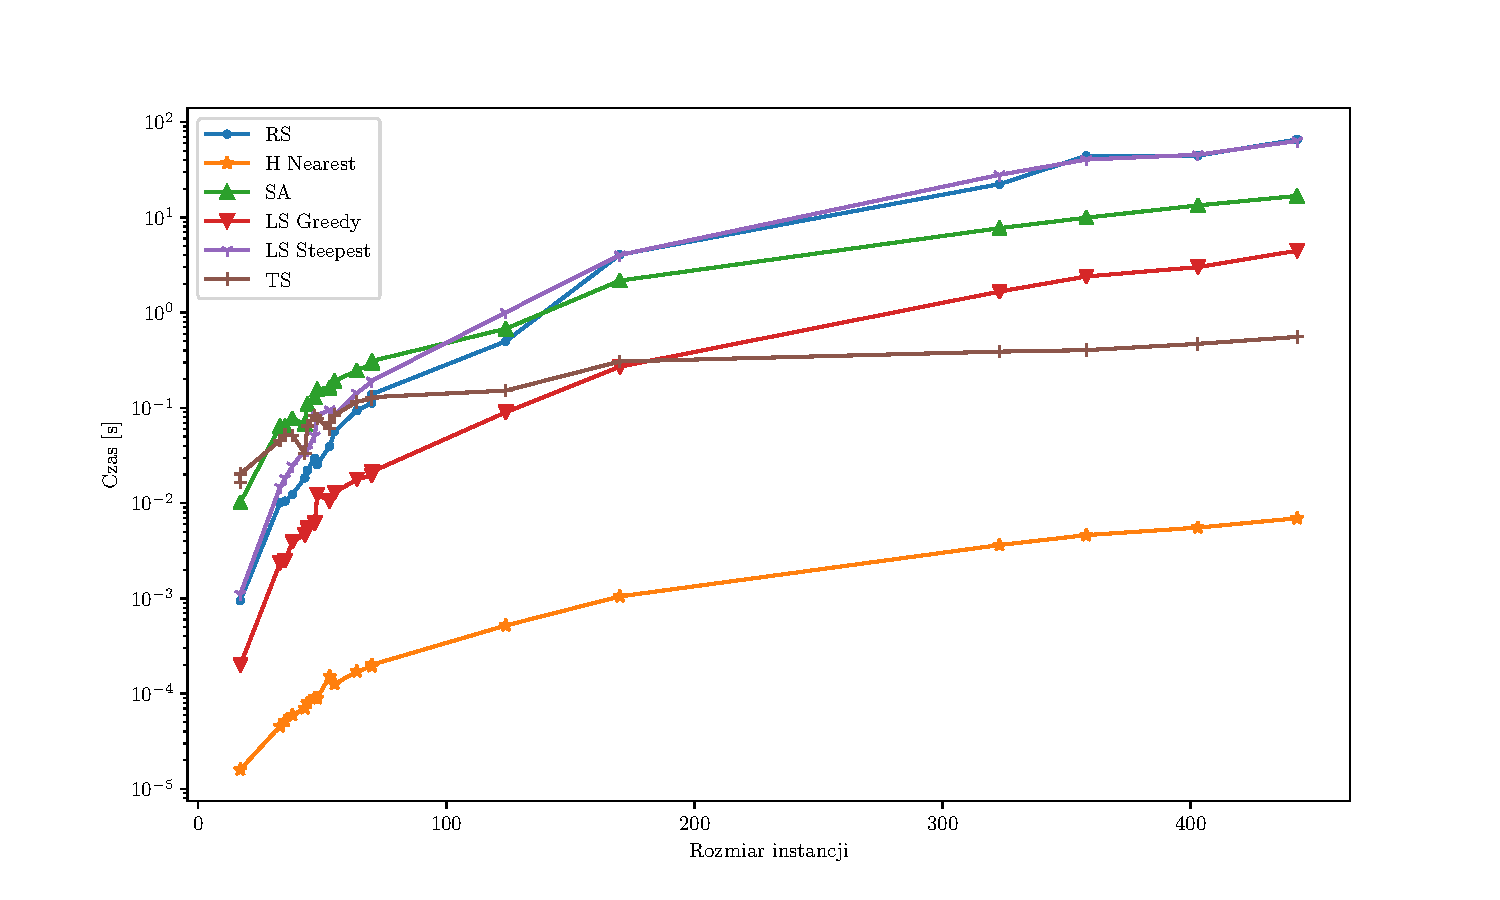
\includegraphics[width=1\textwidth]{plot_mean_time.pdf}
\end{center}
\caption{Czas działania algorytmów}
\label{fig:plot_time}
\end{figure}

\subsection{Efektywność}

Aby zbadać który algorytm jest najbardziej efektywny biorąc pod uwagę czas działania oraz jakoś wyniku wykreśliliśmy wykres który przedstawia te zależności.. Z rys. \ref{fig:plot_quality} można wyczytać że najlepsze wyniki w czasie uzyskał algorytm heurystyczny a najgorsze algorytm losowy.

\begin{figure} 
\begin{center}
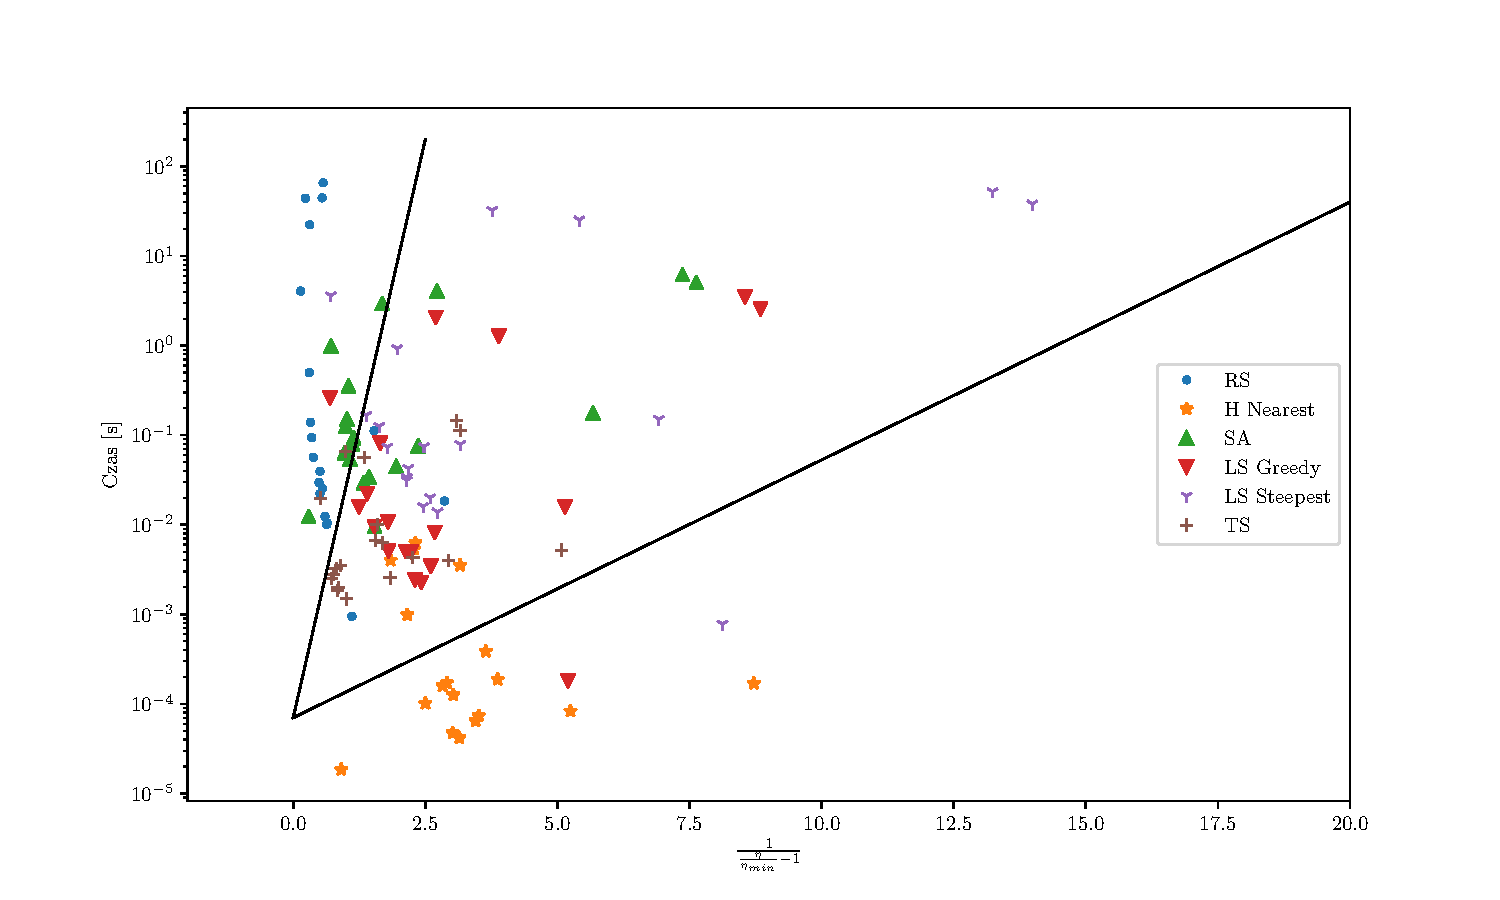
\includegraphics[width=1\textwidth]{quality.pdf}
\end{center}
\caption{Efektywność algorytmów}
\label{fig:plot_quality}
\end{figure}

\subsection{Średnia liczba kroków algorytmów}

\ref{fig:plot_steps}

\begin{figure} 
\begin{center}
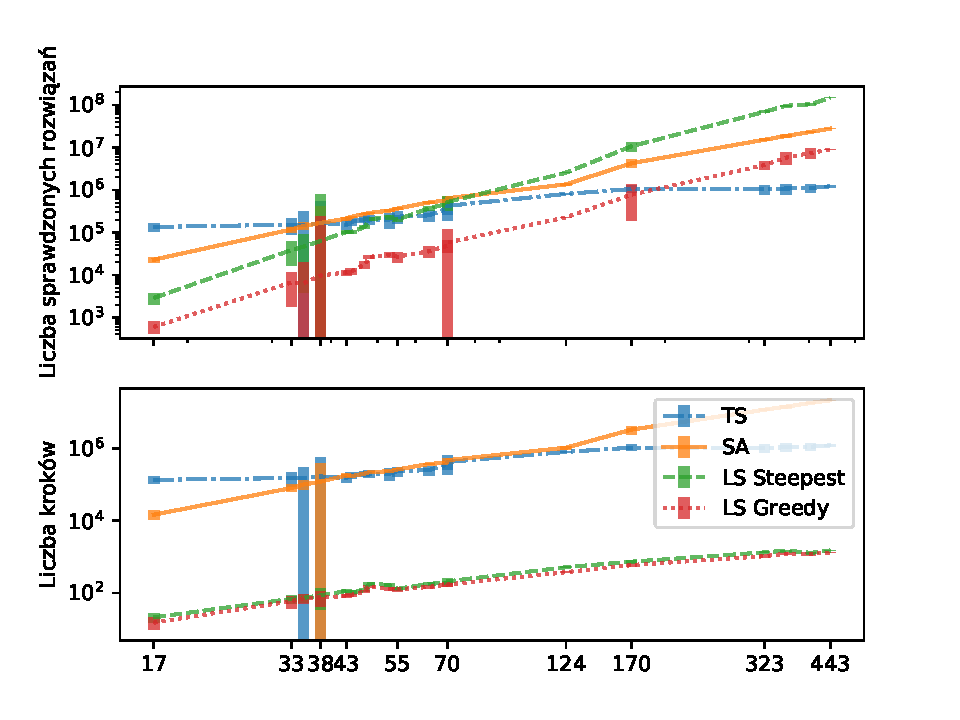
\includegraphics[width=1\textwidth]{steps.pdf}
\end{center}
\caption{Średnia liczba kroków algorytmów}
\label{fig:plot_steps}
\end{figure}

\section{Jakość rozwiązania początkowego, a jakość rozwiązania końcowego}


\begin{figure}
    \begin{center}
        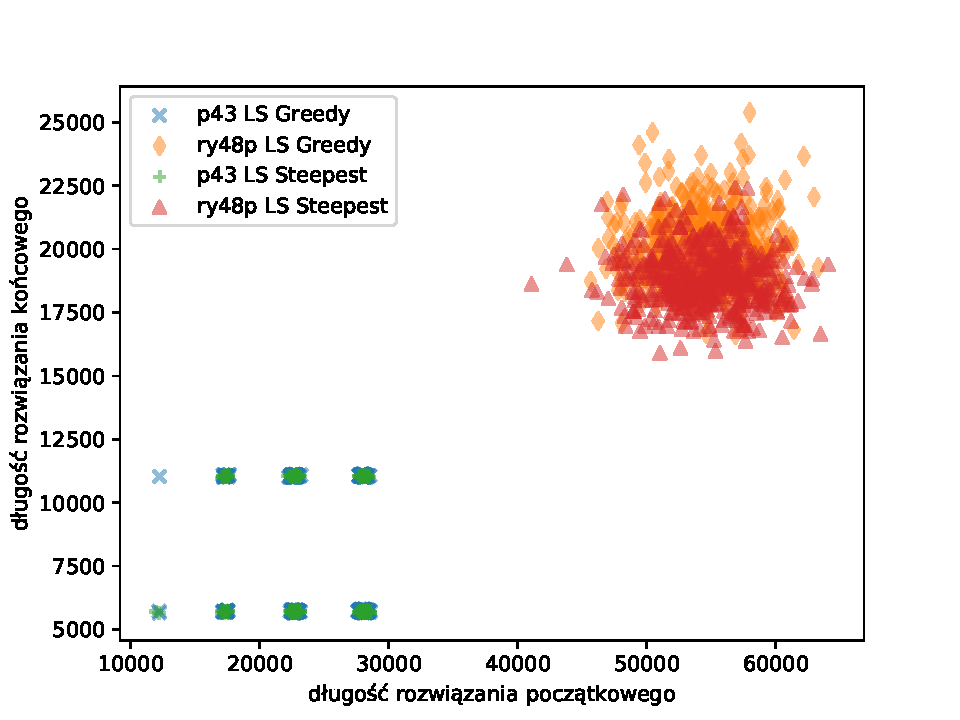
\includegraphics[width=1\textwidth]{first_last_finest.pdf}
    \end{center}
    \caption{Jakość rozwiązania początkowego, a jakość rozwiązania końcowego}
    \label{fig:plot_steps}
\end{figure}

\section{Jakość rozwiązania w zależności od ilości uruchomień}


\begin{figure}
    \begin{center}
        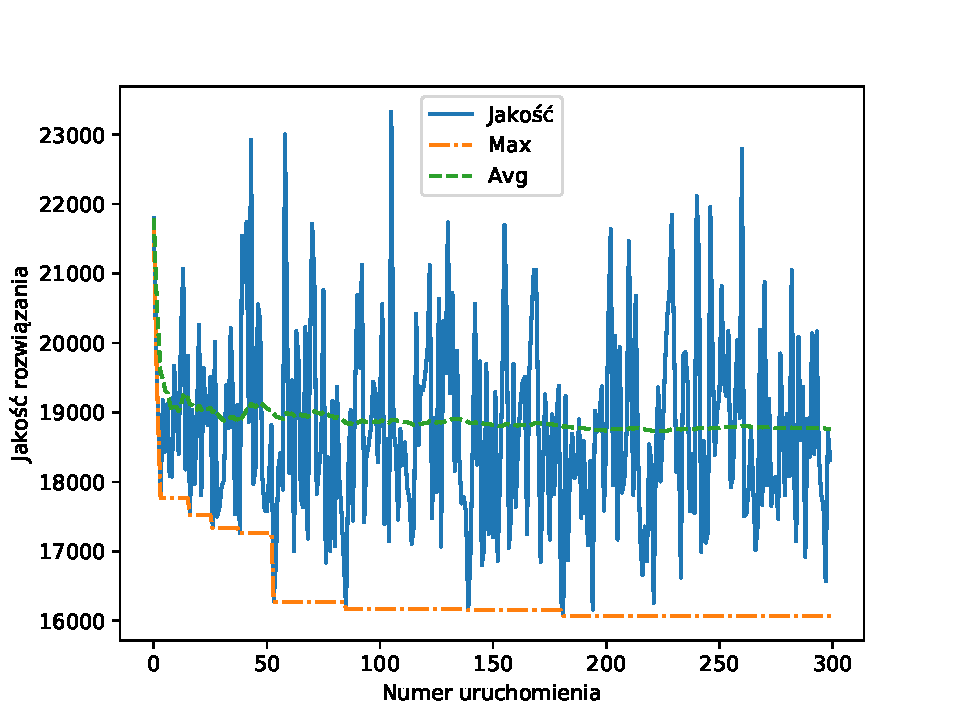
\includegraphics[width=1\textwidth]{multi_run_ry48p_atsp.pdf}
    \end{center}
    \caption{Jakość rozwiązania w zależności od ilości uruchomień. Instancja ry48p.}
    \label{fig:plot_multi_run_ry48p}
\end{figure}

\begin{figure}
    \begin{center}
        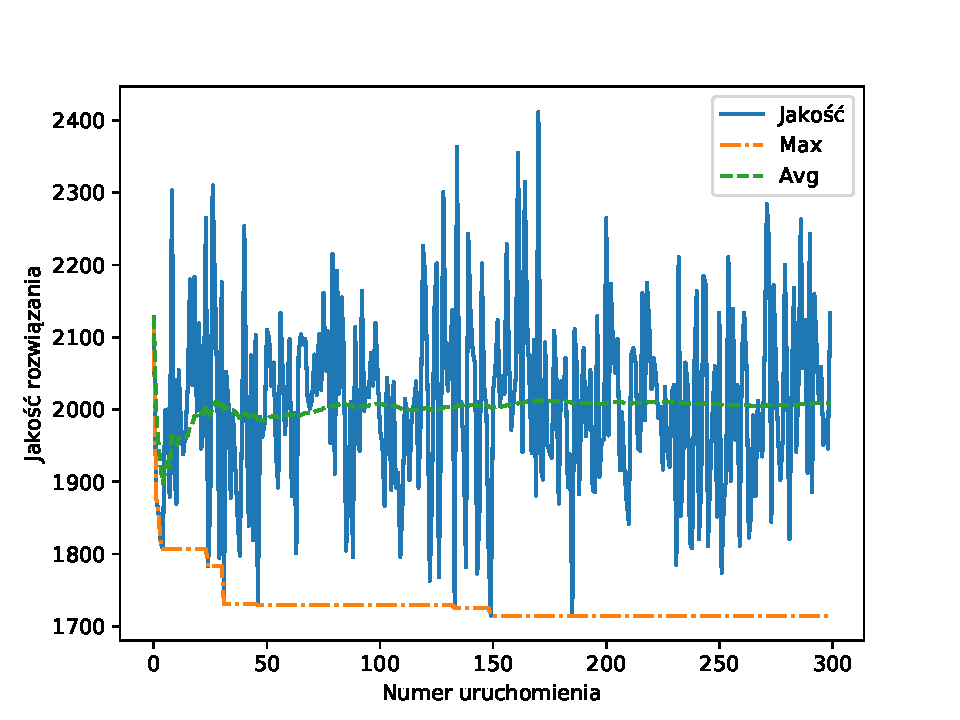
\includegraphics[width=1\textwidth]{multi_run_ftv35_atsp.pdf}
    \end{center}
    \caption{Jakość rozwiązania w zależności od ilości uruchomień. Instancja ftv35.}
    \label{fig:plot_multi_run_ry48p}
\end{figure}


\section{Podobieństwo rozwiązań}

\begin{figure}
    \begin{center}
        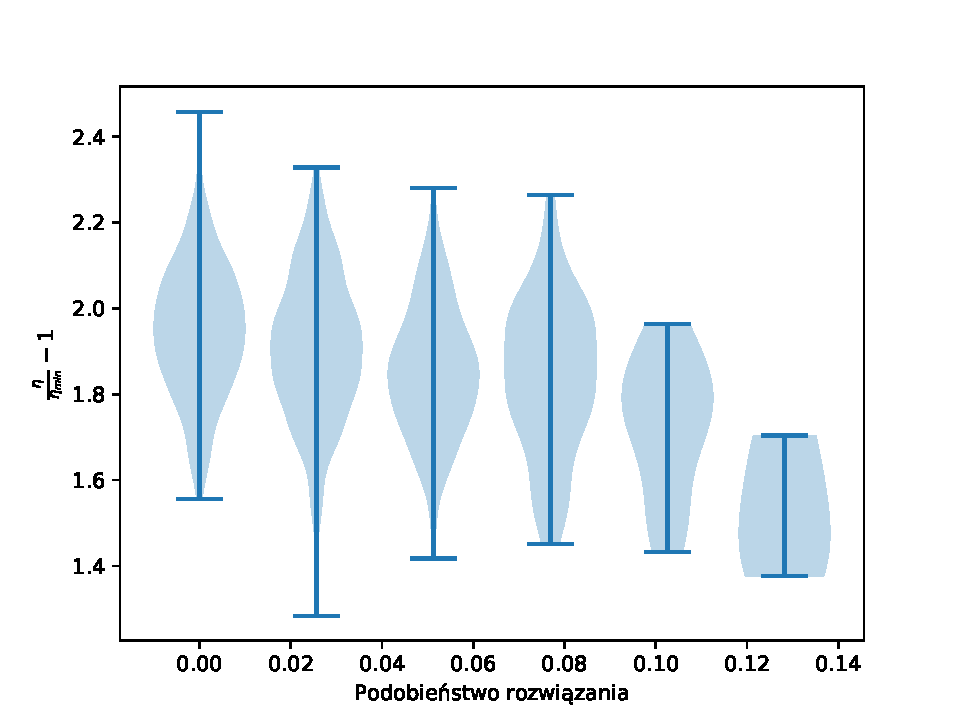
\includegraphics[width=1\textwidth]{quality_similarity_ftv38.pdf}
    \end{center}
    \caption{Jakość rozwiązania w zależności podobieństwa do znalezionego optimum. Instancja ftv38.}
    \label{fig:quality_sim_ftv38}
\end{figure}

\begin{figure}
    \begin{center}
        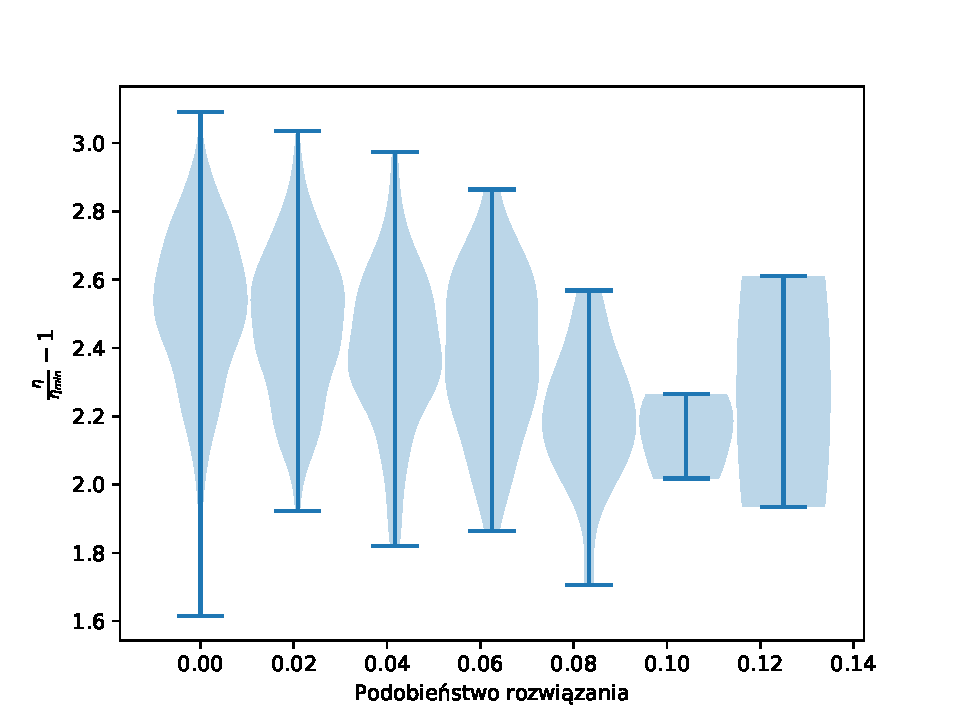
\includegraphics[width=1\textwidth]{quality_similarity_ry48p.pdf}
    \end{center}
    \caption{Jakość rozwiązania w zależności podobieństwa do znalezionego optimum. Instancja ry48p.}
    \label{fig:quality_sim_ry48p}
\end{figure}

\section{Wnioski}

\section{Trudności i problemy}

\section{Propozycje udoskonaleń}

\clearpage

\bibliography{report}
\bibliographystyle{plainurl}


\end{document}
